\documentclass{report}
\usepackage[T1]{fontenc}
\usepackage [utf8]{inputenc}
\usepackage{hyperref}
\usepackage[english]{babel}
\usepackage{amsmath}
\usepackage[a4paper, total={6in, 8in}]{geometry}
\usepackage{graphics}
\usepackage{tgbonum}
\begin{document}
\def\blankpage{%
      \clearpage%
      \thispagestyle{empty}%
      \addtocounter{page}{-1}%
      \null%
      \clearpage}

      % notes:
      % Where should we have background section?
      % Should each chapter (e.g. NMT) have its own background section?
      % 
      % 

\pagenumbering{Roman}
\tableofcontents

%\begin{abstract}

%\end{abstract}


\pagenumbering{arabic}
\chapter{Introduction}

\chapter{Neural Machine Translation (NMT)}
\label{ch:nmt}
Given that there was limited work leveraging BERT for NMT, there were many attemptes including:
\begin{enumerate}
	\item  Use BERT to initialize downstream models and then fine-tuning the models following Devlin et al (2019), e.g. use BERT as encoder for the model, then fine tune it. Unfortunately, this method did not lead to significant improvement.
	\item Use BERT as context-aware embeddings for downstream models following Peters et al (2018). This strategy outperformed the previous one.
	\item Use BERT \item Feed BERT output to all layers instead of using it as embedding only.
\end{enumerate}
In our model, we follow a special case from the third approach. For more details, check \hyperref[ch:our-model]{Our model chapter}.

In the following sections, we get more information about BERT, Transformers and the model of BERT-NMT (combination between both previous architectures).

\section{Background}
\label{sec:nmt-background}
Neural Machine Translation (NMT) achieves a tremendous success in both academic and industry fields. It models the translation process by a  holistic neural network based on encoder-decoder kframework. LSTMs were achieving state-of-art results untill introducing Transformer (Vaswani et al 2017).

Generally, recent models are divided into the following main parts:
\begin{itemize}
	\item Word embedding: A distributional representation for for individual words.
	\item Encoder: Maps input sequence into hidden representation.
	\item Decoder: Maps hidden representation into output sequence. This sequence is a list of probabilities for each word from target language. These probabilities are then used via beam search algorithm to construct output sentences.
\end{itemize}
\section{Bidirectional Encoder Representations from Transformers (BERT)}
\label{sec:bert}
BERT is designed to pre-train deep bidirectional representations from unlabeled text by jointly conditioning on both left and right context in all layers. As a result, the pre-trained BERT model can be fine-tuned with just one additional output layer to create state-of-the-art models for a wide range of tasks, such as question answering and language inference, without substantial task- specific architecture modifications.

Language model pre-training has been shown to be effective for improving many natural language processing tasks (Dai and Le, 2015; Peters et al., 2018a; Radford et al., 2018; Howard and Ruder, 2018). These include sentence-level tasks such as natural language inference (Bowman et al., 2015; Williams et al., 2018) and paraphrasing (Dolan and Brockett, 2005), which aim to predict the relationships between sentences by analyzing them holistically, as well as token-level tasks such as named entity recognition and question answering, where models are required to produce fine-grained output at the token level (Tjong Kim Sang and De Meulder, 2003; Rajpurkar et al., 2016) .

There are two existing strategies for applying pre-trained language representations to downstream tasks: feature-based and fine-tuning. The feature-based approach, such as ELMo (Peters et al., 2018a), uses task-specific architectures that include the pre-trained representations as addi- tional features. The fine-tuning approach, such as the Generative Pre-trained Transformer (OpenAI GPT) (Radford et al., 2018), introduces minimal task-specific parameters, and is trained on the downstream tasks by simply fine-tuning all pre-trained parameters. The two approaches share the same objective function during pre-training, where they use unidirectional language models to learn general language representat ions.

BERT is a fine-tuning based approach. BERT alleviates the previously mentioned unidirectionality constraint by using a “masked lan- guage model” (MLM) pre-training objective, in- spired by the Cloze task (Taylor, 1953). The masked language model randomly masks some of the tokens from the input, and the objective is to predict the original vocabulary id of the masked word based only on its context. Unlike left-to- right language model pre-training, the MLM objective enables the representation to fuse the left and the right context, which allows pre-training a deep bidirectional Transformer. In addition to the masked language model, we also use a “next sentence prediction” task that jointly pre-trains text-pair representations. 

BERT is conceptually simple and empirically powerful. It obtains new state-of-the-art results on eleven natural language processing tasks, including pushing the GLUE score to 80.5% (7.7% point absolute improvement), MultiNLI accuracy to 86.7% (4.6% absolute improvement), SQuAD v1.1 question answering Test F1 to 93.2 (1.5 point absolute improvement) and SQuAD v2.0 Test F1 to 83.1 (5.1 point absolute improvement).

\subsection{Background}
\label{ssec:bert-background}
There is a long history of pre-training general language representations, and we briefly review the most widely-used approaches in this subsection.

\subsubsection{Unsupervised Feature-Based Approaches}
\label{sssec:bert-unsupervised-feature-based-approaches}
Learning widely applicable representations of words has been an active area of research for decades, including non-neural (Brown et al., 1992; Ando and Zhang, 2005; Blitzer et al., 2006) and neural (Mikolov et al., 2013; Pennington et al., 2014) methods. Pre-trained word embeddings are an integral part of modern NLP systems, offering significant improvements over embeddings learned from scratch (Turian et al., 2010). To pre- train word embedding vectors, left-to-right lan- guage modeling objectives have been used (Mnih and Hinton, 2009), as well as objectives to discriminate correct from incorrect words in left and right context (Mikolov et al., 2013) .
These approaches have been generalized to coarser granularities, such as sentence embeddings (Kiros et al., 2015; Logeswaran and Lee, 2018) or paragraph embeddings (Le and Mikolov, 2014). To train sentence representations, prior work has used objectives to rank candidate next sentences (Jernite et al., 2017; Logeswaran and Lee, 2018), left-to-right generation of next sentence words given a representation of the previous sentence (Kiros et al., 2015), or denoising auto-encoder derived objectives (Hill et al., 2016).

ELMo and its predecessor (Peters et al., 2017, 2018a) generalize traditional word embedding research along a different dimension. They extract context-sensitive features from a left-to-right and a right-to-left language model. The contextual representation of each token is the concatenation of the left-to-right and right-to-left representations. When integrating contextual word embeddings with existing task-specific architectures, ELMo advances the state of the art for several major NLP benchmarks (Peters et al., 2018a) including ques- tion answering (Rajpurkar et al., 2016), sentiment analysis (Socher et al., 2013), and named entity recognition (Tjong Kim Sang and De Meulder, 2003). Melamud et al. (2016) proposed learning contextual representations through a task to predict a single word from both left and right context using LSTMs. Similar to ELMo, their model is feature-based and not deeply bidirectional. Fedus et al. (2018) shows that the cloze task can be used to improve the robustness of text generation models .

\subsubsection{Unsupervised Fine-Tuning Approaches}
\label{sssec:bert-unsupervised-fine-tuning-approaches}
As with the feature-based approaches, the first works in this direction only pre-trained word embedding parameters from unlabeled text (Col- lobert and Weston, 2008) .

More recently, sentence or document encoders which produce contextual token representations have been pre-trained from unlabeled text and fine-tuned for a supervised downstream task (Dai and Le, 2015; Howard and Ruder, 2018; Radford et al., 2018). The advantage of these approaches is that few parameters need to be learned from scratch. At least partly due to this advantage, OpenAI GPT (Radford et al., 2018) achieved previously state-of-the-art results on many sentence-level tasks from the GLUE benchmark (Wang et al., 2018a). Left-to-right language modeling and auto-encoder objectives have been used for pre-training such models (Howard and Ruder, 2018; Radford et al., 2018; Dai and Le; 2015).

\begin{figure}
	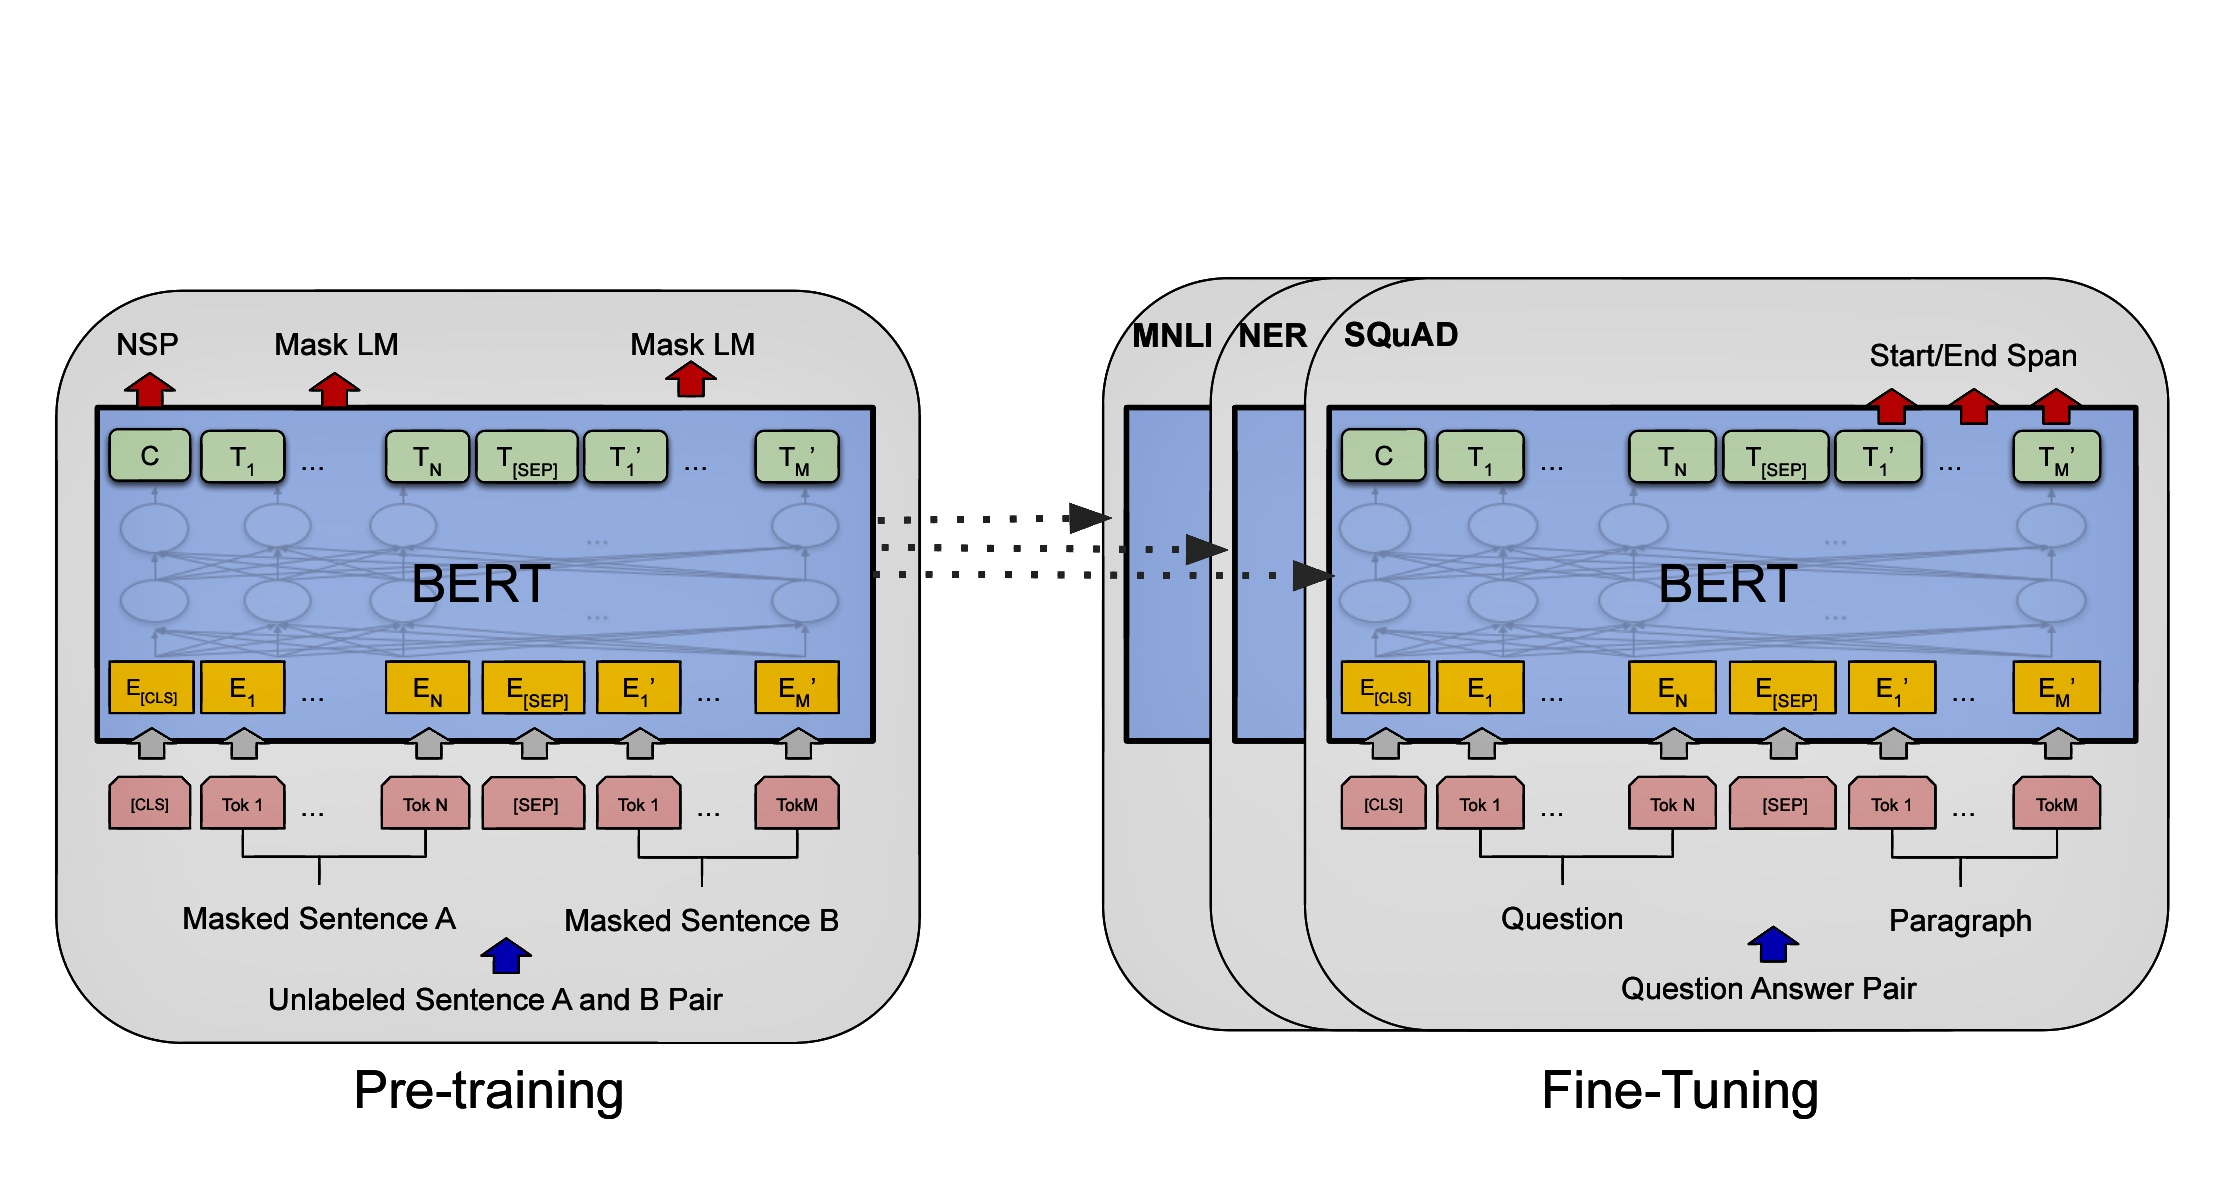
\includegraphics{images/bert/overall-pre-training-and-fine-tuning-procedures.jpg}
	\caption{Overall pre-training and fine-tuning procedures for BERT. Apart from output layers, the same architectures are used in both pre-training and fine-tuning. The same pre-trained model parameters are used to initialize models for different down-stream tasks. During fine-tuning, all parameters are fine-tuned. [CLS] is a special symbol added infromt of every input example, and [SEP] is a special separator token (e.g. separating questions/answers)}
	\label{fig:overall-training-procedure-for-bert}
\end{figure}

\subsubsection{Transfer Learning From Supervised Data}
\label{sssec:bert-transfer-learning}
There has also been work showing effective transfer from supervised tasks with large datasets, such as natural language inference (Conneau et al., 2017) and machine translation (McCann et al., 2017). Computer vision research has also demonstrated the importance of transfer learning from large pre-trained models, where an effective recipe is to fine-tune models pre-trained with ImageNet (Deng et al., 2009; Yosinski et al., 2014) .

\subsection{BERT Implementation}
\label{ssec:bert-implementation}
Here, we consider, in details, BERT and its implementation. There are two steps in this framework pre-training and fine-tuning. During pre-training, the model is trained on unlabelled data over a different pre-training tasks. For fine-tuning, the BERT model is first initialized with the pre-trained parameters, and all of the parameters are fine-tuned using labelled data from the downstream tasks. Each downstream task has separate fine-tuned models, even though they are initialized with the same pre-trained parameters. The question-answering example in figure \ref{fig:overall-training-for-bert} will serve as a running example for this subsection.

A distinctive features of BERT is its unified architecture across different tasks. There is minimal difference between the pre-trained architecture and the final downstream architecture.

\textit{Model Architecture}
BERT's model architecture is a multi-layer bidirectional transformer encoder based on the original implementation described in Vaswaani et al., 2017 and released in the \href{https://github.com/tensorflow/tensor2tensor}{tensor2tensor library}. Because the use of transformers has become common and the implementation is almost identical to the original, we will omit an exhaustive background description from this section and you can reach \hyperref[sec:transformer]{transformer section} as well as excellent guides such as \href{http://nlp.seas.harvard.edu/2018/04/03/attention.html}{"The Annotated Transformer."}.

We denote the number of layers (i.e., transformer blocks) as $L$, the hidden size as $H$, and the number of self-attention heads as the feed-forward/filter size to be $4H$, e.g., 3072 for $H=768$ and 4096 for $H=1024$. 
% Note: We note that in the literature, the bidirectional transformer is often referred to as a "transformer encoder", while the left "context" only version is referred to as a "transformer decoder" since it can be used for text generation.

\textit{Input/Output Representation}
To make BERT handle a variety of downstream tasks, the input representation is able to unambigously represent both a single sentence and a pair of sentences (e.g., <question, answer>) in one token sequence. Throughout this section, a "sentence" can be an arbitrary span of contiguous text, rather than an actual linguistic sentence. A "sequence" refers to the input token sequence to BERT, which may be a single sentence or two sentences packed together.

We use wordpiece embeddings (Wu et al., 2016) with a 30,000 token vocabulary. The first token of every sequence is always a special classification token ([CLS]). The final hidden state corresponding to this token is used as the aggregate sequence representation for classification tasks. Sentence pairs are packed togetherinto a single sequence. We differentiate the sentences in two ways. First, we separate them with a special token ([SEP]). Second, We add a learned embedding to every token indicating whether it belongs to sentence A or sentence B. As shown in figure \ref{fig:overall-training-procedure-for-bert}, we denote input embedding $E$, the final hidden vector of the specil [CLS] token as $C \in R^H$, and the final hidden vector for the $i^{th}$ input token as $T_i \in R^H$.

For a given token, its input representation is constructed by summing the corresponding token, segment , and position embeddings. A visualization of this construction can be seen in figure \ref{fig:bert-input-representation}.

\begin{figure}
	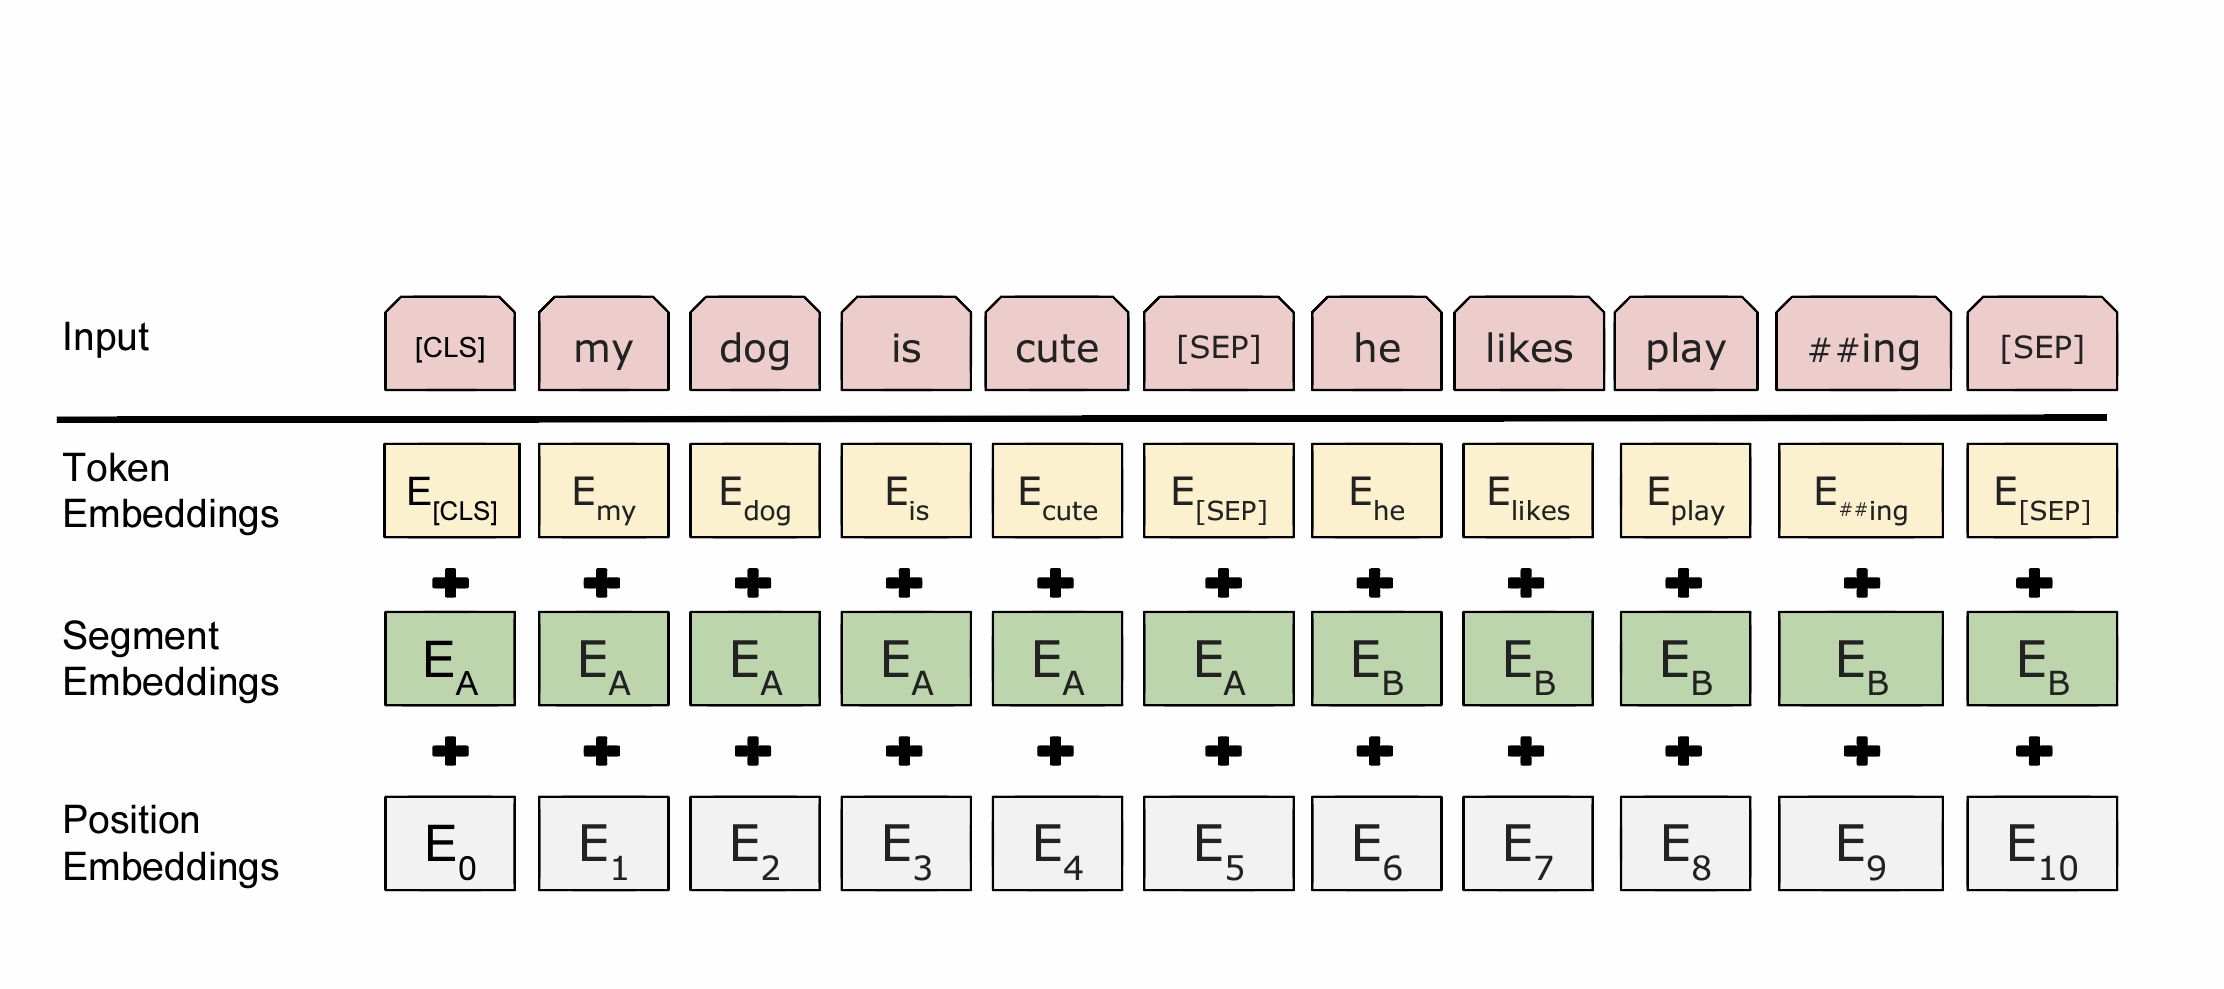
\includegraphics{images/bert/input-representation.jpg}
	\caption{BERT input representation. The input embeddings are the sum of the token embeddings, the segmentation embeddings are the position embeddings.}
	\label{fig:bert-input-representation}
\end{figure}

\subsubsection{Pre-Training BERT}
\label{sssec:pre-training-bert}
Unlike Peters et al., (2018a) and Radford et al., (2018), in BERT, there is no use for traditional left-to-right or right-to-left language models to pre-train the model. Instead, the authors pre-train BERT using two unsupervised tasks. This step is presented in the left part of figure \ref{fig:overall-training-procedure-for-bert}.

\textit{Task 1 Masked LM}:
Intuitively, it is reasonable to believe that a deep bidirectional model is stricctly more powerful than either a left-to-right model or the shallow concatenation of a left-to-right and a right-to-left model. Unfortunately, standard conditional language models can only be trained left-to-right or right-to-left, since bidirectional conditioning would allow each word to directly "see itself", and the model could trivially predict the target word in a multi-layer context.

In order to train a deep bidirectional representation, we simply mask some percentage of the input tokens at random, and then predict those masked tokens. We refer to this procedure as a "Masked LM" (MLM), although it is often referred to as a Cloze task in the literature (Taylor, 1953). In this case, the final hidden vectors corresponding to the mask tokens are fed into an output softmax over the vocabulary, as in a standard LM. In all of their experiments, they mask 15\% of all workpiece tokens in each sequence at random. In contrast to denoising auto-encoders (Vincent et al., 2008), they only predict the masked words rather than reconstructing the entire input.

Although this allows us to optain a bidirectional pre-trained model, a downside is that we are creating a mismatch between pre-training and fine-tuning, since the [MASK] token doesn't appear during fine-tuning. To mitigate this, they do not always replace "masked" words with the actual [MASK] token. The training data generator chooses 15\% of the token positions at random for prediction. If the $i-th$ token is chosen, they replace the $i-th$ token with:
\begin{enumerate}
	\item The [MASK] token 80\% of the time
	\item A random token 10\% of the time
	\item The unchanged $i-th$ token 10\% of the time
\end{enumerate}

\textit{Task 2 Next Sentence Prediction (NSP)}
Many important downstream tasks such as Question Answering (QA) and Natural Language Inference (NLI) are based on understanding the relationship between two sentences, which is not directly captured by language modeling. In order to train a model that understands sentence relationships, they pre-train for a binarized next sentence prediction task that can be trivially generated from any monolingual corpus. Specifically, when choosing the sentences A and B for each pre-training example, 50\% of the time B is the actual next sentence that follows A (labelled as [IsNext], and 50\% of the time it is a random sentence from the corpus labelled as [NotNext]. As shown in figure \ref{fig:overall-training-procedure-for-bert}, C is used for next sentence prediction (NSP).The NSP task is closely related to representation-learning objectives used in Jernite et al., (2017) and Logeswaran and Lee (2018). However, in prior work, only sentence embeddings are transferred to downstream tasks, where BERT transfers all parameters to initialize end-task model parameters.

\subsubsection{Fine-Tuning BERT}
\label{sssec:fine-tuning-bert}Fine-tuning is straightforward since the self-attention mechanism in the transformer $T$ allows BERT to model many downstream tasks-- whether they involve single text or text pairs -- by swapping out the appropriate inputs and outputs. For applications involving text pairs, a common pattern is to independently encode text pairs before applying bidirectional cross attention, such as Parikh et al, (2016); Seo et al, (2017). BERT instead uses the self-attention mechanisms to unify these two stages, as encoding a concatenated text pair with self-attention effectively includs bidirectional cross attention between two sentences.

For each task, we simply plug  in the task-specific inputs and outputs into BERT and fine-tune all the parameters end-to-end. At the input, sentence A and sentence B from pre-training are analogous to:
\begin{enumerate}
	\item Sentence pairs in paraphrasing
	\item Hypothesis-premise pairs in entailment
	\item Question-passage pairs in Question Answering, and
	\item Degenerate text-$\phi$ pair in text classification or sequence tagging.
\end{enumerate}
At the output, the token representations are fed into an output layer for token-level tasks, such as sequence tagging or question answering, and the [CLS] representation is fed into an output layer for classification, such as entailment or sentiment analysis.

Compared to pre-training, fine-tuning is relatively inexpensive. All of the results can be replicated in at most one hour on a single Cloud TPU, or a few hours on a GPU, starting from the exact same pre-trained model. 

\section{Transformers}
\label{sec:transformers}
First introduced by (Vaswani et al., 2017) as a replacement for state-of-the-art Neural Network architectures: Recurrent Neural Network (RNN), Long Short Term Memory (LSTM) and Gated Recurrent Unit (GRU). Recurrent models typically factor computation along the symbol positions of the input and output sequences. Aligning the positions to steps in computation time, they generate a sequence of hidden states $h_t$, as a function of the previous hidden state $h_{t-1}$ and the input for position $t$. This inherently sequential nature precludes parallelization within training examples, which becomes critical at longer sequence lengths, as memory constraints limit batching across examples. 
In this section, we discuss Transformer as introduced in "Attention Is All You Need!" paper (Vaswani et al., 2017). 
Transformer: It is a model architecture eschewing recurrence and instead relying entirely on an attention mechanism to draw global dependencies between input and output. The Transformer allows for significantly more parallelization and can reach a new state of the art in translation quality after being trained for a relatively short period of time compared to RNNs, LSTMs and GRUs.

\subsection{Background}
\label{ssec:transformers-background}
Self-attention, sometimes called intra-attention is an attention mechanism relating different positions of a single sequence in order to compute a representation of the sequence. Self-attention has been used successfully in a variety of tasks including reading comprehension, abstractive summarization, textual entailment and learning task-independent sentence representations.

\subsection{Model Architecture}
\label{ssec:transformers-model-architecture}
Most competitive neural sequence transduction models have an encoder-decoder structure. Here, the encoder maps an input sequence of symbol representations $(x_1,...,x_n)$ to a sequence of continuous representations $z = (z_1,...,z_n)$. Given $z$, the decoder then generates an output sequence $(y_1, ..., y_m)$ of symbols one element at a time. At each step the model is auto-regressive, consuming the previously generated symbols as additional input when generating the nextT
The Transformer follows this overall architecture using stacked self-attention and point-wise, fully connected layers for both the encoder and decoder, shown in the left and right halves of figure \ref{fig:transformer-model-architecture}, respectively.
\begin{figure}
	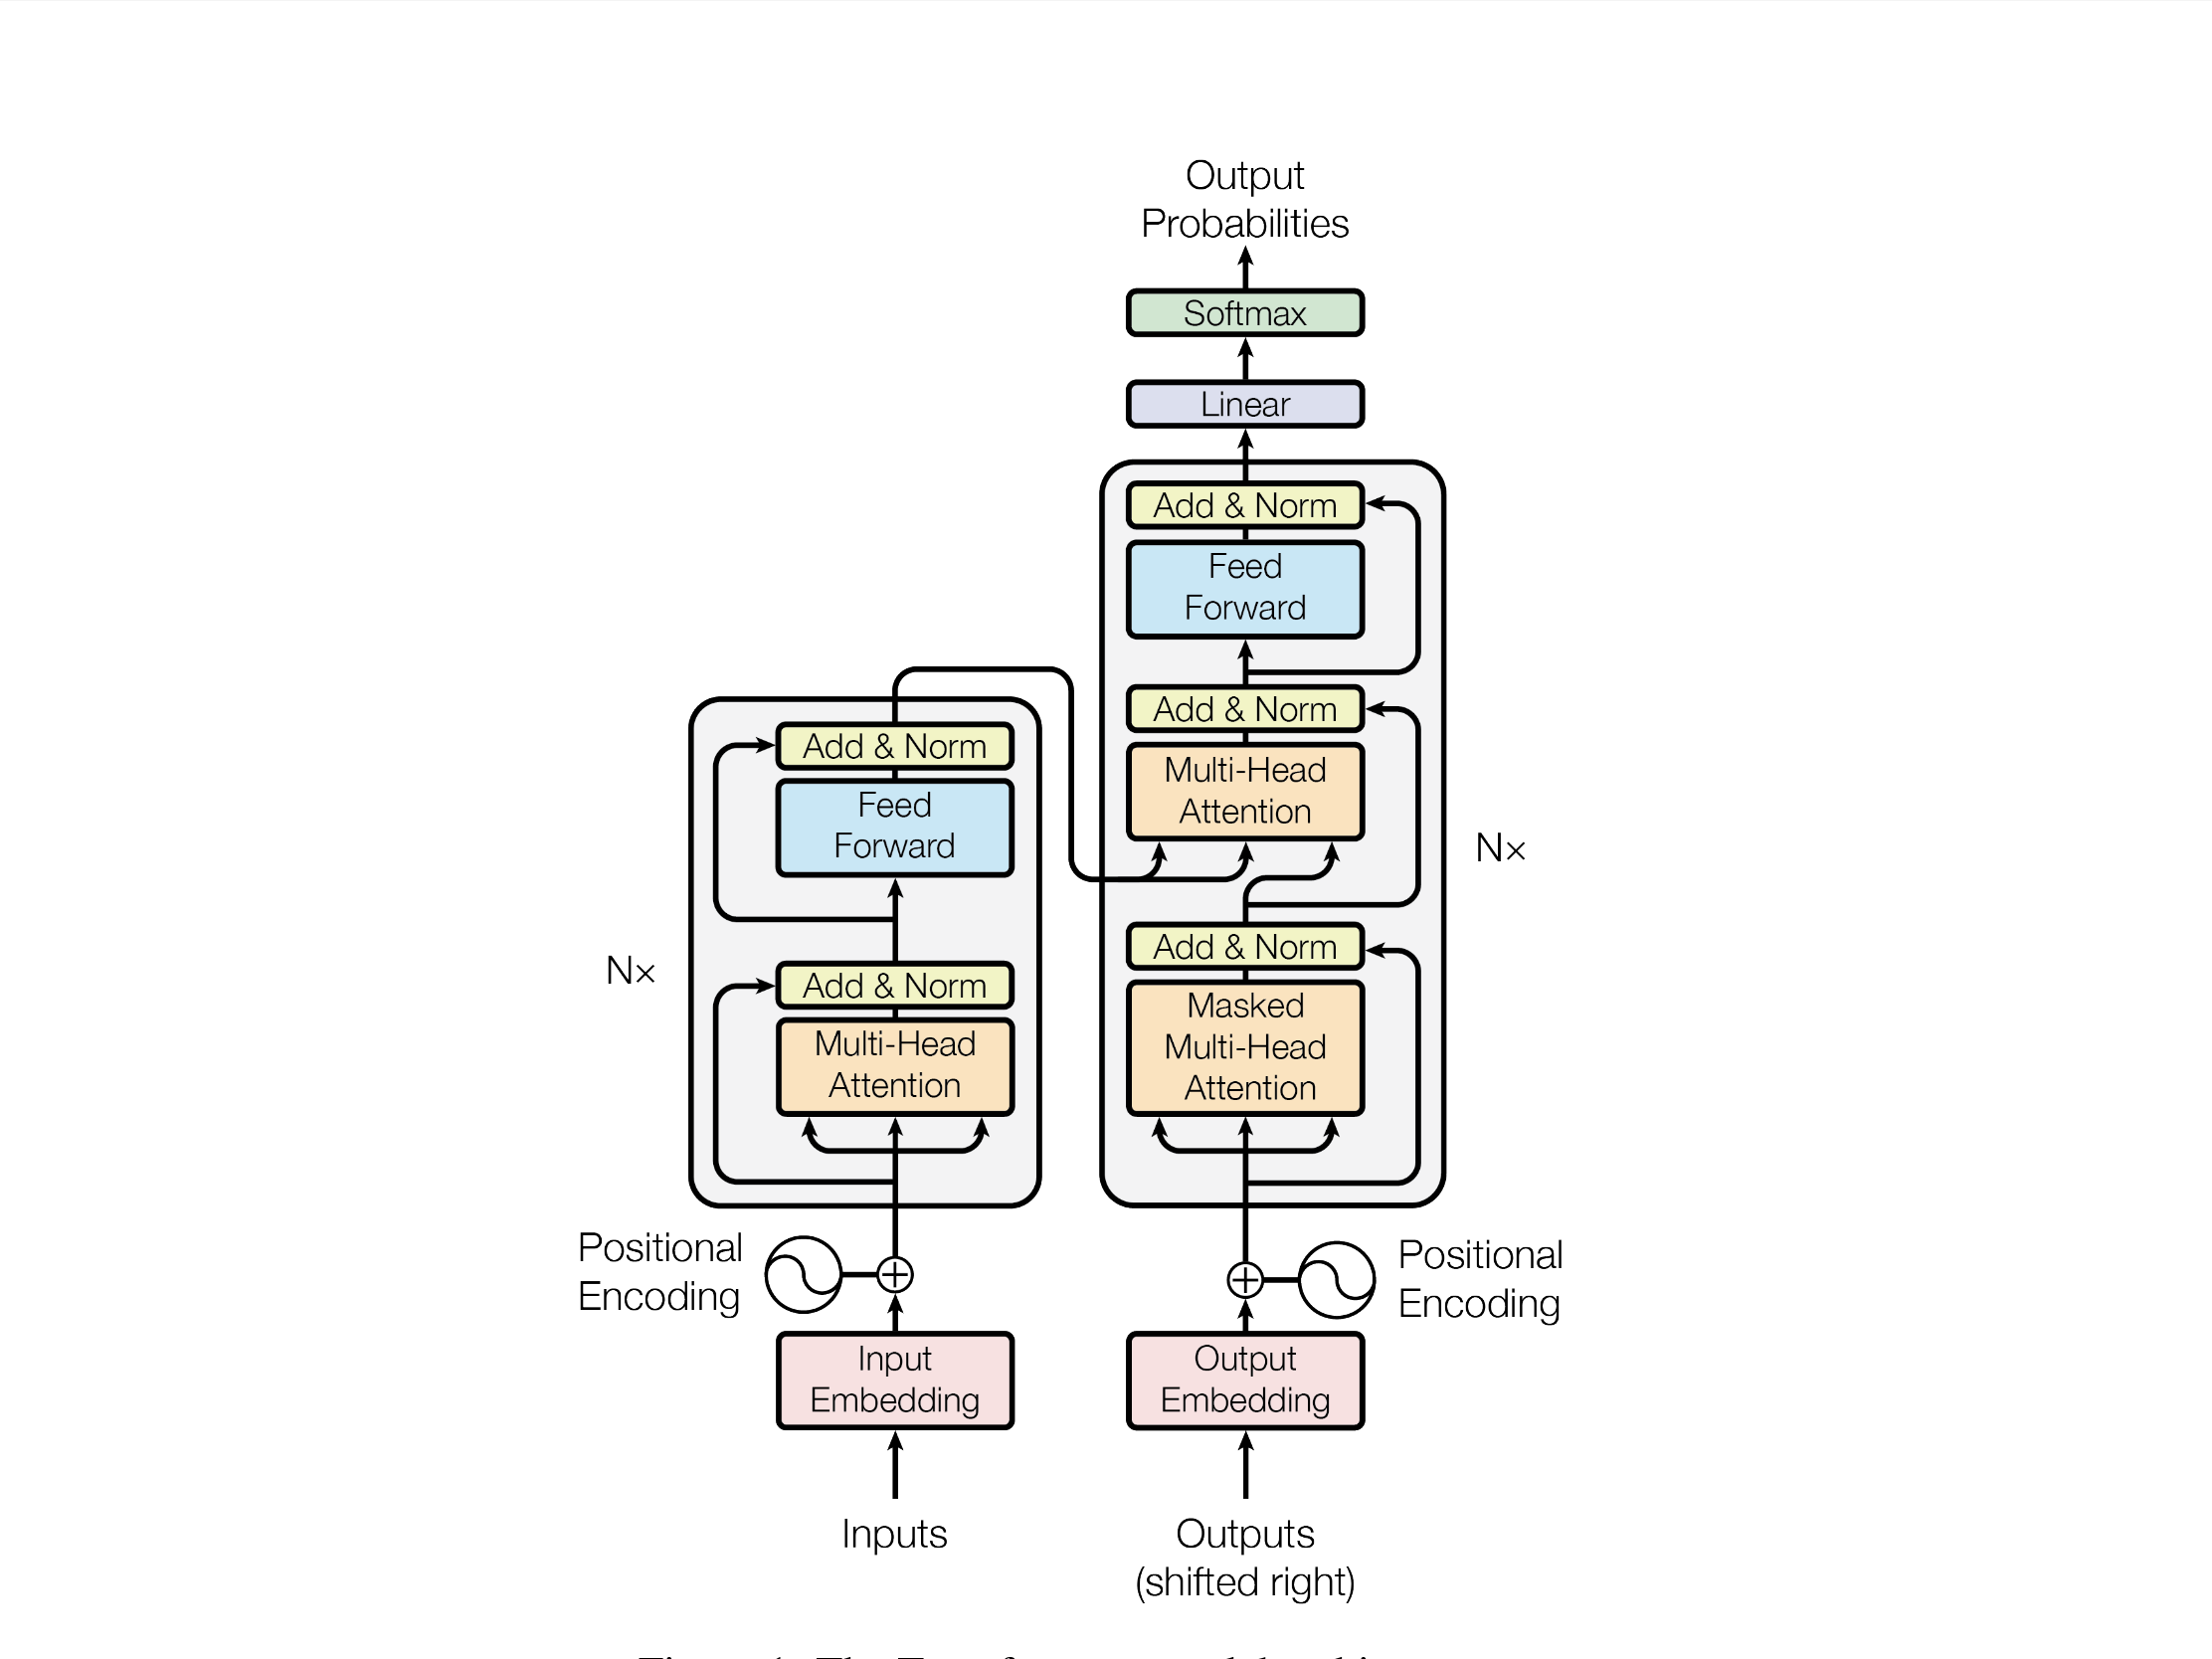
\includegraphics{images/transformer/model-architecture.PNG}
	\caption{Transformer Model Architecture}
	\label{fig:transforer-model-architecture}
\end{figure}

\subsubsection{Encoder And Decoder Stacks}
\label{sssec:transformer-enc-dec-stacks}
\textit{Encoder}: The encoder is composed of a stack of $N = 6$ identical layers. Each layer has two sub-layers. The first is a multi-head self-attention mechanism, and the second is a simple, position-wise fully connected feed-forward network. We employ a residual connection around each of the two sub-layers, followed by layer normalization. That is, the output of each sub-layer is $LayerNorm(x + Sublayer(x))$, where $Sublayer(x)$ is the function implemented by the sub-layer itself. To facilitate these residual connections, all sub-layers in the model, as well as the embedding layers, produce outputs of dimension $dmodel = 512$. 

\textit{Decoder}: The decoder is also composed of a stack of $N = 6$ identical layers. In addition to the two sub-layers in each encoder layer, the decoder inserts a third sub-layer, which performs multi-head attention over the output of the encoder stack. Similar to the encoder, we employ residual connections around each of the sub-layers, followed by layer normalization. We also modify the self-attention sub-layer in the decoder stack to prevent positions from attending to subsequent positions. This masking, combined with fact that the output embeddings are offset by one position, ensures that the predictions for position i can depend only on the known outputs at positions less than $i$.

\subsubsection{Attention}
\label{sssec:transformer-attention}
An attention function can be described as mapping a query and a set of key-value pairs to an output, where the query, keys, values, and output are all vectors. The output is computed as a weighted sum of the values, where the weight assigned to each value is computed by a compatibility function of the query with the corresponding key.

\textit{Scaled DOT-Product Attention}
As shown in figure \ref{fig:scaled-dot-product-attention}, the input consists of queries and keys of dimension $d_k$, and values of dimension $d_v$. We compute the dot products of the query with all keys, divide each by $\sqrt{d_k}$, and apply a softmax function to optain the weights on the values.
\begin{figure}
	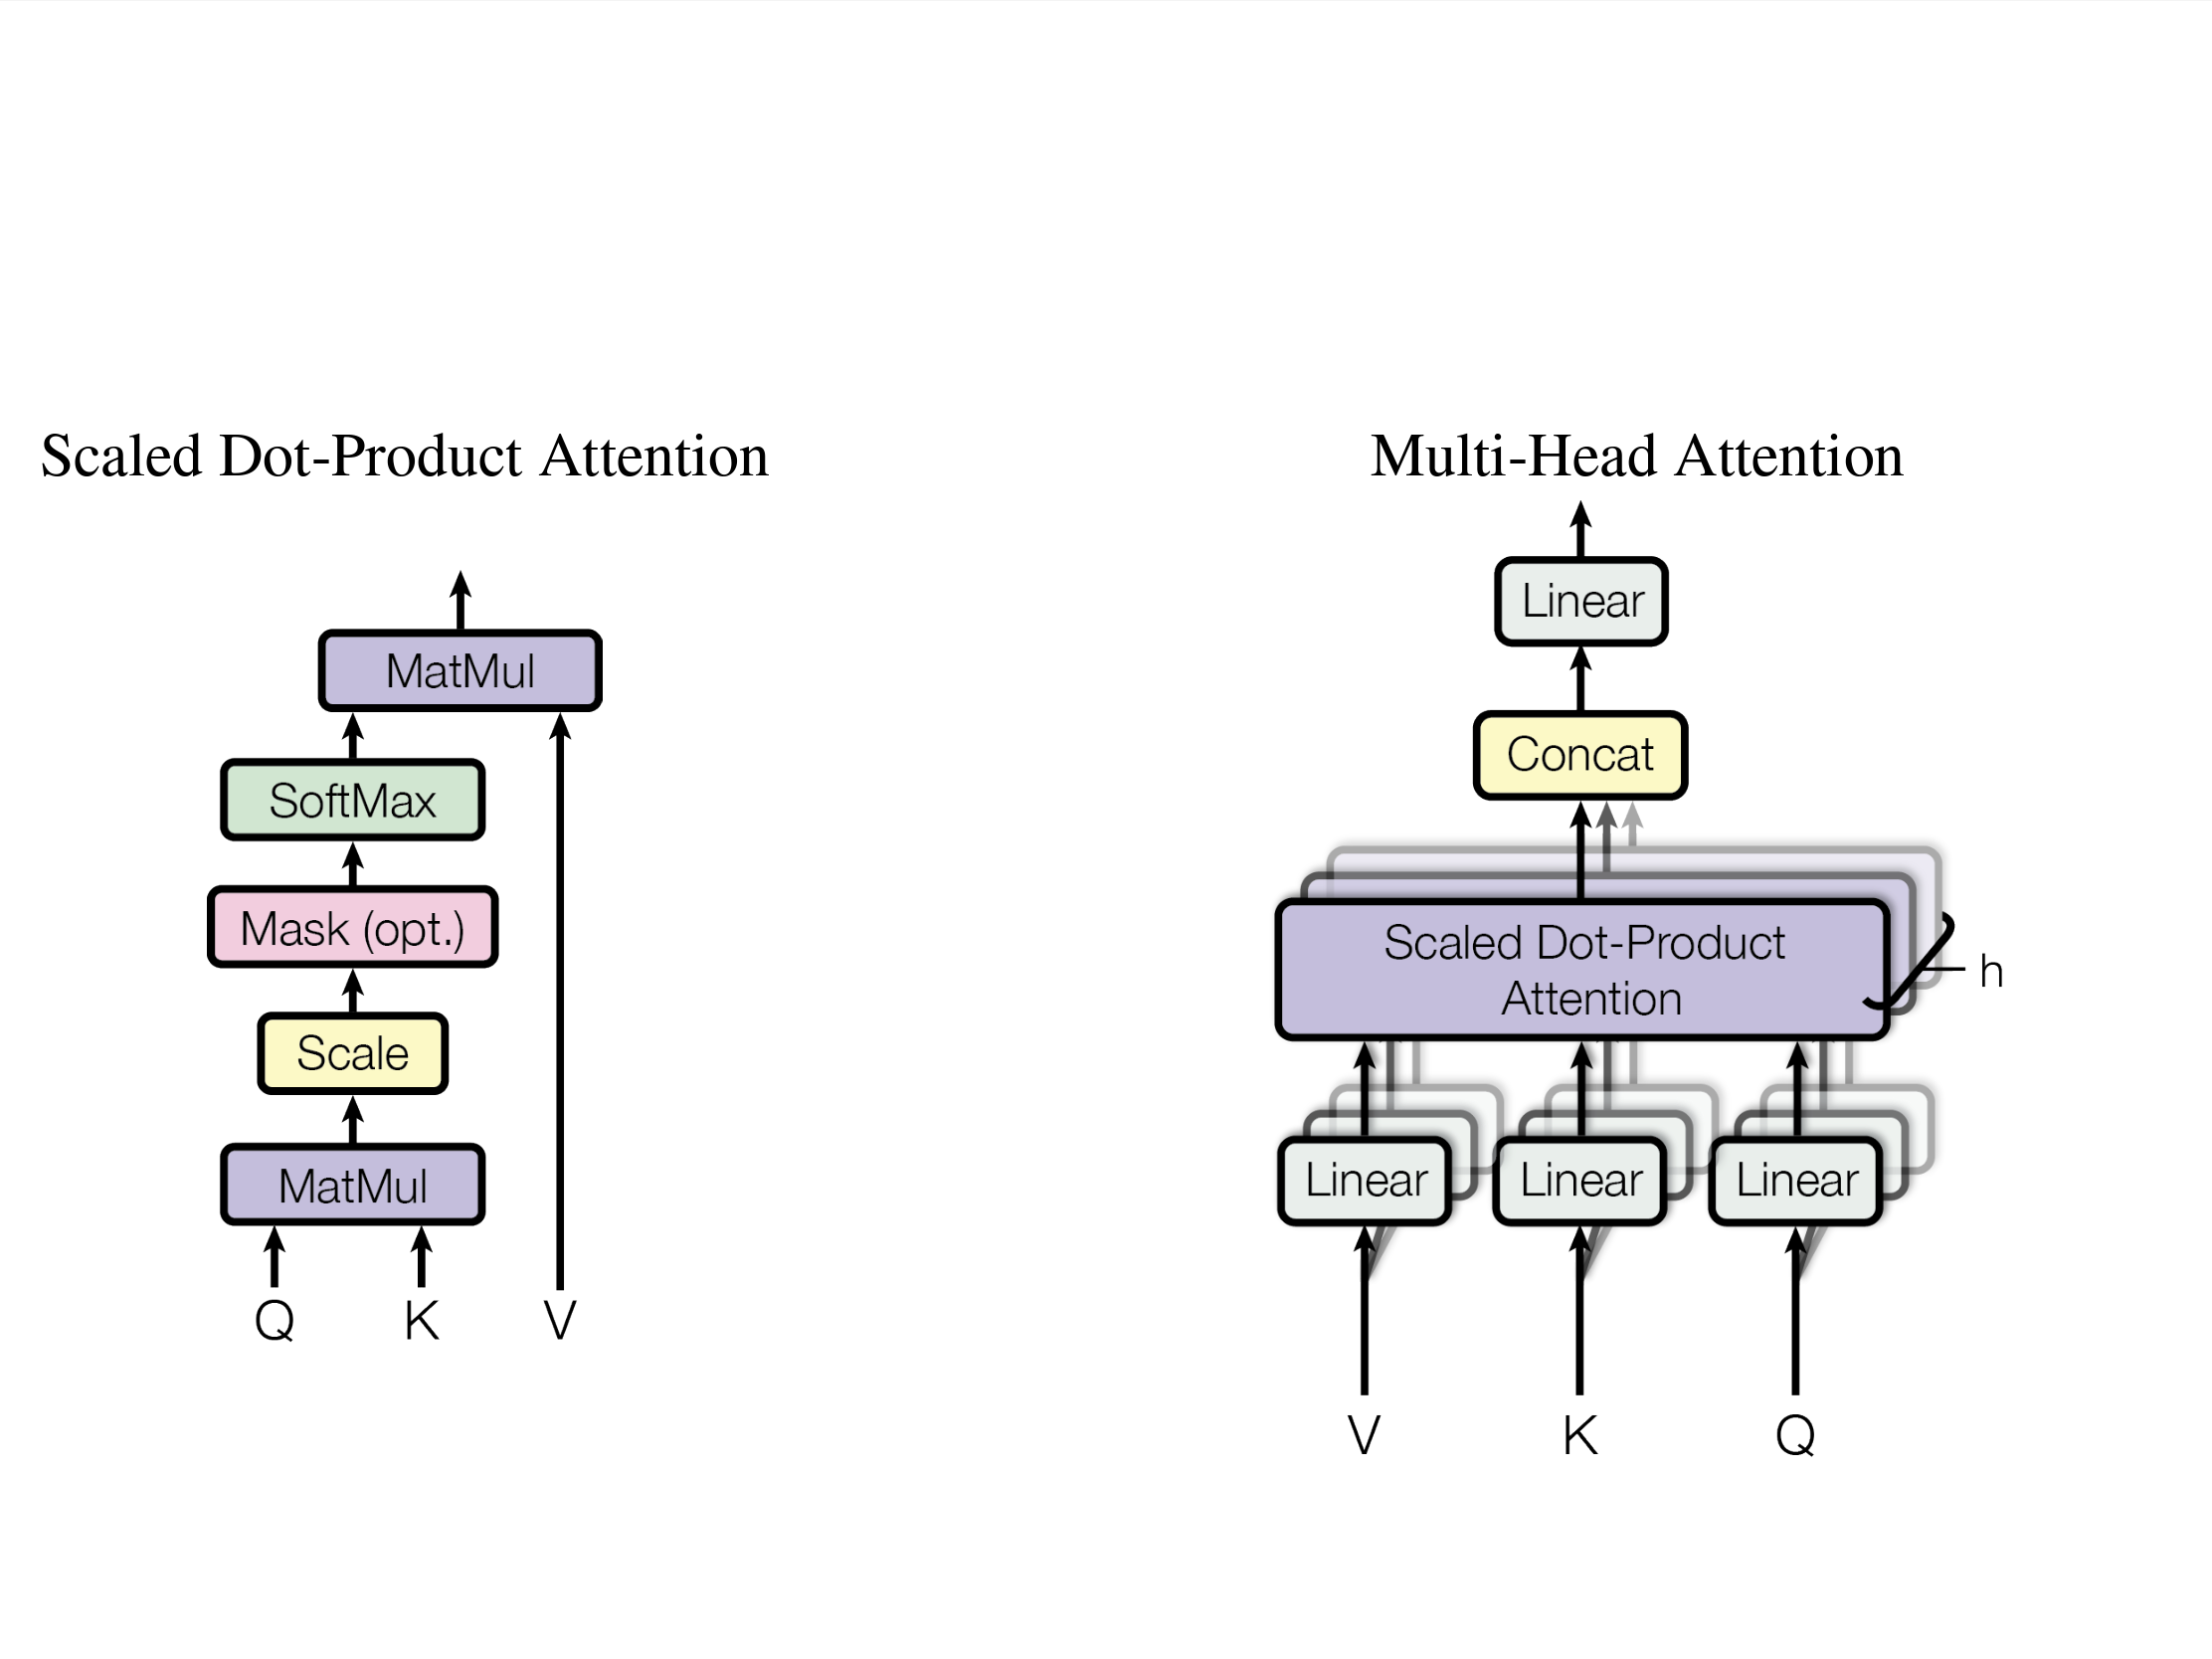
\includegraphics{images/transformer/scaled-dot-product-attention.PNG}
	\caption{(Left) Scaled Dot-Product Attention. (Right) Multi-Head Attention consists of several attention layers running in parallel.}
	\label{fig:scaled-dot-product-attention}
\end{figure}
In practice, we compute the attention function on a set of queries simultaneously, packed together into a matrix $Q$. The keys and values are also packed together into matrices $K$ and $V$. We compute the matrix of outputs as:
\begin{equation}
	Attention(Q, K, V) = softmax(\frac{Q K^T}{\sqrt{d_k}}V) %Equation 1
	\label{eq:transformer-attention}
\end{equation}
The two most commonly used attention functions are Additive attention and Dot-Product (Multiplicative) attention. Dot-Product attention is identical to the current algorithm, except for the scaling factor of $\frac{1}{\sqrt{d_k}}$. Additive attention computes the compatibility function using a feed-forward network with a single hidden layer. While the two are similar in theoretical complexity, Dot-Product attention is much faster and more space-efficient in practice, since it can be implemented using highly optimized matrix multiplication code.

While for small values of $d_k$, the two mechanisms perform similarly, additive attention outperforms Dot-Product attention without scaling for larger values of $d_k$. We suspect that for large values of $d_k$, the Dot-Products grow large in magnitude, pushing the softmax function into regions where it has extremely small gradients. To counteract this effect, we scale the Dot-Products by $\frac{1}{\sqrt{d_k}}$.

\textit{Multi-head Attention}:
Instead of performing a single attention function with $d_{model}-dimensional keys$, values and queries it is found that beneficial to linearly project the queries, keys and values $h$ time with different, learned linear projections to $d_k, d_k and d_v$ dimensions respectively. On each of these projected versions of queries, keys and values we then perform the attention function in parallel, yielding $d_v$-dimensional output values. These are concatenated and once again projected, resulting in the final values, as depicted in figure \ref{fig:scaled-dot-product-attention}.

Multi-head attention allows the model to jointly attend to information from different representation subspaces at different positions. With a single attention head, averaging inhibits this.

\begin{equation*}
	\begin{aligned}
	Multihead(Q, K, V)=contact(head_1,...,head_h)W^O
	where head_i=attention(Q W_i^Q, K W_i^K, V W_i^V)
\end{aligned}
\end{equation*}

Where the projection are parameter matrices $W_i^Q \in R^{d_{model} \times d_k}$, $W_i^k \in R^{d_{model} \times d_k}$, $W_i^V \in R^{d_{model} \times d_v}$ and $W^O \in R^{h d_v \times d_{model}}$.

In this model, they employ $h=8$ parallel attention layers, or heads. For each of these, we use $d_k=d_v=d_{model}/h=64$. Due to the reduced dimension of each head, the total computational cost is similar to single-head attention with full dimensionality.

\textit{Application of attention in the model}
The transformer uses multi-head attention in three different ways:
\begin{itemize}
	\item In "Encoder-Decoder attention" layers, the queries come from the previous decoder layer, and the memory keys and values come from the output of the encoder. This allows every position in the decoder to attend over all positions in the input sequence. This mimics the typical encoder-decoder attention mechanisms in sequence-to-sequence models.
	\item The encoder contains self-attention layers. In a self-attention layer, all of the keys, values and queries come from the same place, in this case, the output of the previous layer in the encoder. Each position in the encoder can attend to all positions in the previous laye of the encoder.
	\item Similarly, self-attention layers in the decoder allow each position in the decoder to attend to all positions in the decoder up to and including the position. We need to prevent leftward information flow in the decoder to preserve the auto-regressive property. We implement this inside of scaled Dot-Product attention by masking out (setting to $-\infty$) all values in the input of the softmax which correspond to illegal connection. See figure \ref{fig:scaled-dot-product-attention}. %figure 2 in transformer
\end{itemize}
	
\subsubsection{Position-Wise Feed-Forward Networks}
\label{sssec:transformer-position-wise-ffn}
n addition to attention sub-layers, each of the layers in the encoder and decoder contains a fully connected feed-forward network, which is applied to each position separately and identically. This consists of two linear transformations with a ReLU activation in between.
\begin{equation}
	FFN(x)=max(0, x W_1 + b_1) + W_2 + b_2 %equation 2
	\label{eq:transformer-ffn}
\end{equation}
While the linear transformations are the same accross different positions, they use different parameters from layer to layer. Another way of describing this is as two convolutions with kernel size 1. The dimensionality of input and output is $d_{model}=512$, and the inner-layer has dimensionality $d_{ff}=2048$.

\subsubsection{Embeddings And Softmax}
\label{sssec:transformer-embedding-and-softmax}
Similar to other sequence transduction models, this model uses learned embeddings to convert the input tokens and output tokens to vectors of dimension $D_{model}$. We also use the usual learned linear transformation and softmax function to convert the decoder output to predicted next-token probabilities. In this model, the same weight matrix is shared between the two embedding layers and the pre-softmax linear transformation,. In the embedding layers,we multiply those weight by $\sqrt{d_{model}}$.

\subsubsection{Positional Encoding}
\label{sssec:transformer-positional-encoding}
Since this model contains no recurrence and no convolution, in order for the model to make use of the order of the sequence, we must inject some information about the relative or absolute position of the tokens in the sequence. To this end, we add "Positional Encodings" to the input embeddings at the bottom of the encoder and decoder stacks. The positional encodings have the same dimension $d_{model}$ as the embeddings, so that the two can be summed. There are many choices of positional encodings learned and fixed.

We use sine and cosine functions of different frequencies:
\begin{equation*}
	\begin{aligned}
		PE_{(POS, 2i)}=sin(POS/10000^{2i/d_{model}}) \\
		PE_{(POS, 2i+1)}=cos(POS/10000^{2i/d_{model}})
\end{aligned}
\end{equation*}
where $POS$ is the position and $i$ is the dimension. That is, each dimension of the positional encoding corresponds to a sinusoid. The wave length from a geometric progression from $2\pi to 10000 \dot 2\pi$. This function is chosen because hypothesizing it would allow the model to easily learn to attend by relative positions, since for any fixed offset $k$, $PE_{POS+k}$ can be represented as a linear function of $PE_{POS}$.

\iffalse
\subsection{Wy Self-Attention}
\label{ssec:transformer-why-self-attention}
In this subsection, we compare various aspects of self-attention layers to the recurrent and convolutional layers commonly used for mapping one variable-length sequence of symbol representation $(x_1, ..., X_n)$ to another sequence of equal length $(z_1, ..., z_n)$, with $x_i, z_i \in R^d$, such as a hidden layer in a typical sequence transduction encoder or decoder. Motivating the use of self-attention, we consider three desiderata.

One is the total computational complexity per layer. Another is the amount of computation that can be parallelized, as measured by the minimum number of sequential operations required.

The third is the path-length between long-range dependencies in the network. Learning long-range dependencies is a key challenge in many sequence transduction tasks. One key factor affecting the ability to learn such dependencies is the length of the pathes forward and backward signals have to traverse in the network. The shorter these pathes between any combination of positions in the input and output sequences, the easier it is to learn long-range dependencies. Hence, we also compare the maximum path length between any two input and output positions in networks composed of the different layers types.

As noted in table 1
\fi

\section{BERT-fused Model}
\label{sec:bert-nmt}
In this section, we discuss the architecture introduced by Jinhua et al, (2020) in "Incorporating BERT inNeural Machine Translation" paper. After the preliminary exploration of using BERT as con- textual embedding, it is found that it is better than using BERT for fine-tuning. They propose a new algorithm named BERT-fused model, in which they first use BERT to extract rep- resentations for an input sequence, and then the representations are fused with each layer of the encoder and decoder of the NMT model through attention mechanisms. After conducting experiments on supervised (including sentence-level and document-level translations), semi-supervised and unsupervised machine translation, and achieve state-of-the-art results on seven benchmark datasets. OThe code is available at \href{https://github.com/bert-nmt/bert- nmt}{BERT-NMT github repo}.

\subsection{Algorithm}
\label{ssec:bert-nmt-algorithm}
In BERT-fused model, we exploit the representation from BERT by feeding it into all layers rather than served as input embeddings only. We use the attention mechanism to adaptively control how each layer interacts with the representations, and deal with the case that BERT module and NMT module might use different word segmentation rules, resulting in different sequence (i.e., representation) lengths. Compared to standard NMT, in addition to BERT, there are two extra attention modules, the BERT-encoder attention and BERT-decoder attention. An input sequence is first transformed into representations processed by BERT. Then, by the BERT- encoder attention module, each NMT encoder layer interacts with the representations obtained from BERT and eventually outputs fused representations leveraging both BERT and the NMT encoder. The decoder works similarly and fuses BERT representations and NMT encoder representations.

Notations: 
\begin{itemize}
	\item Let $X$ and $Y$ denote the source and language domain and target language domain respectively, which are the collections of sentences with corresponding languages.
	\item For any sentence $x \in X$ and $y \in Y$, let $l_x$ and $l_y$ denote the number of units (e.g., words or sub-words) in $x$ and $y$. 
	\item The $i-th$ unit in $x/y$ denoted as $x_i /y_i$.
	\item Denote the encoder, decoder and BERT as Enc, Dec and BERTd respectively.
	\item For ease of reference, we call the encoder and decoder as the $NMT module$.
	\item W.l.o.g., we assume both the encoder and decoder consists of $L$ layers.
	\item Let $attn(q, K, V)$denote the attention layer, where $q, K$ and $V$ indicate query, key and value respectively(Vaswani et al., 2017).
	\item We use the same feed-forward layer as that used in (Vaswaani et al., 2017) and denote it as $FFN$.
	\item Mathematical formulation of the above layers are left at % \hyperref[sec:transformers]{transformers section}.
\end{itemize}

\subsubsection{The Model}
\label{sssec:bert-fused-the-model}
An illustration of the algorithm is shown in figure \ref{fig:fig:bert-fused-architecture}.
\begin{figure}[h] %revise
	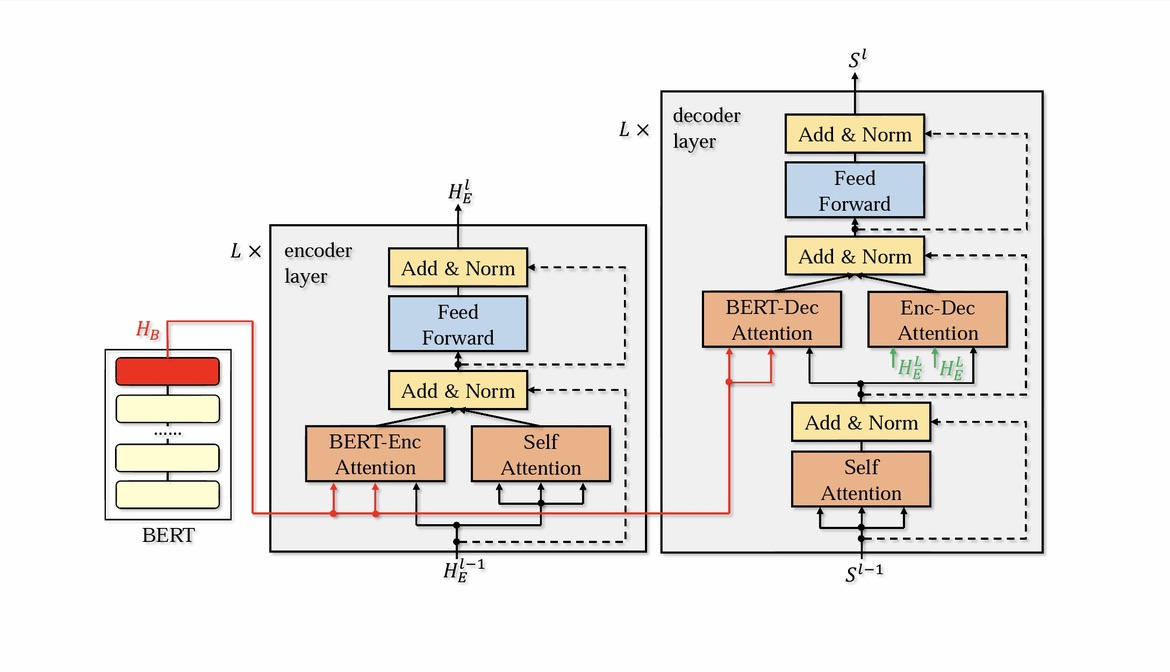
\includegraphics{images/bert-fused-model/architecture.jpeg}
	\caption{The architecture of BERT-fused model. The left and write figures represeents the BERT, encoder and decoder respectively. Dash lines denote residual connections. $H_B(red part) and H_e^L (green part)$ denote the output of the last layer from BERT and encoder.}
	\label{fig:bert-fused-architecture}
\end{figure}

Steps of the algorithm:
\begin{enumerate}
	\item Given any input $x \in X$, BERT first encodes it into representation $H_B=BERT(x). H_B$ is the output of last layer in BERt. The $h_{B, i} \in H_B$ is the representation of $i-th$ wordpiece in $x$.
	\item Let $H_E^l$ denote the hidden representation of $l-th$ layer in the encoder, and let $H_E^0$ denote word embedding of sequence $x$. Denote $i-th$ element in $H_E^l$ as $h_i^l$ for any $i \in [l_x]$. In the $l-th$ layer, $l \in [L]$,,
	\begin{equation}
		\tilde{h_i^l}= \frac{1}{2} (attn_S(h_i^{l-1}, H_E^{l-1}, H_E^{l-1}) + attn_B(h_i^{l-1}, H_B, H_B)), \forall i \in [l_x] 
		\label{eq:bert-fused-input-for-new-layer} %equation 1
	\end{equation}
	where $attn_S$ and $attn_B$ are attention models % see equation 6 % link
	with different parameters. Then each $\tilde{h_i^l}$ is further processed by $FFN(.)$ defined in equation %7
	and we get the output of the $l-th$ layer : $H_E^l = (FFN(\tilde{h_1^l}), ..., FFN(\tilde{h_{l_x}^l})$. The encoder will eventually output $_E^L$ from the last layer.
\item Let $S_{<t}^l$ denote the hidden state of $l-th$ layer in the decoder perceeding time step $t$, i.e., $S_{<t}^l = (S_1^l, ..., S_{t-1}^l)$. Note: $S_1^0$ is a special token indicating the start of a sequenceand $S_t^0$ is the embedding of the predicted word at time-step $t-1$. At the $l-th$ layer, we have 
	\begin{equation}
		\begin{aligned}
\hat{S_t^l}= attn_s(S_t^{l-1}, S_{<t-1}^{l-1}, S_{<t-1}^{l-1}); \\
\tilde{S_t^l}= \frac{1}{2}(attn_B(\hat{S_t^l}, H_B, H_B) + attn_E(\hat{S_t^l}, H_E^L, H_E^l)), S_t^l = FFN(\tilde{S_t^l} %continue 
\label{eq:bert-fused-hidden-state} %equation 2 
	\end{aligned}
	\end{equation}
\end{enumerate}

The $attn_S$, $attn_B$ and $attn_E$ represent self-attention model, BERT-decoder attention model and encoder-decoder attention model respectively. Equation (2) % previous one
iterates over layersand we can eventuallyt optain $S_t^L$. Finally, $S_t^L$ is mapped via a linear transformation and softmax to get the $t-th$ predicted word $\hat{y_t}$. The according process continuous until meeting the end-of-sentence token.
In this framework, the output of BERT serves as an external sequence representation, and we use an attention model to incorporate it into the NMT model. This is a general way to leverage the pre-trained model regardless of the tokenization way.

\subsubsection{DROP-NET TRICK}
\label{sssec:drop-net-trick}
Inspired by dropout (Srivastava et al., 2014) and drop-path (Larsson et al., 2017), which can regularize the network training. The benefit of this drop-net tric is to ensure that the features output by BERT and the conventional encoder are fully utilized. The drop-net will effect Equation \ref{eq:bert-fused-input-for-new-layer} and Equation \ref{eq:bert-fused-hidden-state}. Denote the drop-net rate as $P_{net} \in [0,1]$. At each training iteration, for any layer $l$, we uniformly sample a random variable $U^l$ from $[0,1]$, then all the $\tilde{h_i^l}$ in Equation \ref{eq:bert-fused-input-for-new-layer} are calculated in the following way:
\begin{equation}
	\begin{aligned}
	\tilde{h_i^l}= I(U^l < \frac{P_{net}}{2}) \dot attn_S(h_i^{l-1}, H_E^{l-1}, H_E^{l-1}) + I(U^l > 1- \frac{P_{net}}{2}) \dot attn_B(h_i^{l-1}, H_B, H_B) \\
	+ \frac{1}{2} I(\frac{P_{net}}{2} \leq U^l \leq 1-\frac{p_{net}}{2}) \dot  (attn_S(h_i^{l-1}, H_E^{l-1}, H_E^{l-1}) + attn_B(h_i^{l-1}, H_B, H_B)) 
	\label{eq:bert-fused-input-for-new-layer-with-drop-net} %equation 3
\end{aligned}
\end{equation}

where $I(.)$ is the indicator function.

For any layer, with probability $\frac{p_{net}}{2}$, either the BERT-encoder attention or self-attention is used only; w.p. (1-$P_{net}$), both the two attention models are used. For example, at a specific iteration, the first layer might uses $attn_S$ only, while the second layer uses $attn_B$ only. During inference time, the expected output of each attention model is used, which is $E_{U~uniform[0,1]}(\tilde{h_{i, drop-net}^l})$. The expression is exactly Equation \ref{eq:bert-fused-input-for-new-layer}. 

Similarly, for training of the decoder, with the drop-net trick, we have:
\begin{equation}
	\begin{aligned}
	\tilde{S_{t, drop-net}^l}=I(U^l < \frac{P_{net}}{2}) \dot attn_B(\hat{S_t^l}, H_B, H_B) + I(U^l > 1- \frac{P_{net}}{2}) \dot attn_E(\hat{S_t^l}, H_E^L, H_E^L) \\
	    + \frac{1}{2} I(\frac{P_{net}}{2} \leq U^l \leq 1-\frac{P_{net}}{2}) \dot (attn_B(\hat{S_t^l}, H_B, H_B) + attn_E(\hat{S_t^l}, H_E^L, H_E^L))
	    \label{eq:bert-fused-hidden-state-with-drop-net} % equation 4
    \end{aligned}
    \end{equation}

    For inference, it is calculated in the same way as Equation \ref{eq:bert-fused-hidden-state}. Using this technique can prevent network from overfitting.

\subsubsection{Discussion}
\label{sssec:bert-fused-discussion}
\textit{Comparison with ELMo}
As introduced in \hyperref[sec:nmt-background]{background section}, ELMo (Peters et al., 2018) provides a context-aware embeddings for the encoder in order to capture richer information of the input sequence. The current approach is a better way of leveraging the features from the pre-trained model:
\begin{enumerate}
	\item The output features of the pre-trained model are fused in all layers of the NMT module, ensuring the well-pre-trained features are fully exploited
	\item We use attention model to bridge the NMT module and the pre-trrained features of BERT, in which the NMT module can adaptively determine how to leverage the features from BERT.
	
\end{enumerate}

\textit{Limitations}
This approach has several limitations:
\begin{enumerate}
	\item Additional storage cost: it leverages a BERT model, which results in additional storage cost. However, considering the BLEU improvement and the fact that we do not need additional training of BERT, we believe that the additional storage is acceptable.
	\item Additional inference time: We use BERT to encode the input sequence, which takes about 45% additional time. % details in appendix C. link to it or mention it.
\end{enumerate}

In the following chapter, we explain in details parameters of our model and testing.

\chapter{Our Model}
\label{ch:our-model}

\section{About The Data}
\label{sec:about-the-data}
In the following table, we represent some statistics about the data used for training :

\begin{center}
	\begin{tabular}{ |c|c|c| }
		\hline
 & Arabic & English \\
Number of sentences (Training) & 262727 & 262727 \\
Number of sentences (Validation) & 65681 & 65681 \\
Number of sentences (Testing) & 82103 & 82103 \\
Total number of words (Training) & 668514 & 6707651 \\
Total number of words (validation) & 145369 & 1654898 \\
Total number of words (testing) & 209003 & 2105851 \\
Number of distinct words (training) & 210696 & 91574\\
Number of distinct words (validation) & 100187 & 42346 \\
Number of distinct words (testing) & 109921 & 46457 \\
number of distinct words including digits (training) & 210696 & 96834 \\
number of distinct words including digits (validation) & 102063 & 44162 \\
number of distinct words including digits (testing) & 111476 & 47986 \\
		\hline
	\end{tabular}
\end{center}

\section{Specifications Of Model And Machine}
\label{sec:our-model-specs}
We have got a virtual machine on Google Cloud Platform (GCP) of the following specifications:
\begin{itemize}
	\item 8 cores vCPUs
	\item 52 GB RAM
	\item 4x Nvidia Tesla T4 GPUs (Total 64 GB), and
	\item 400 GB storage.
\end{itemize}

With these specifications, we were able to run a model of the following configurations:
\begin{itemize}
	\item Architecture: Transformer (Vaswani et al., 2017)
	\item Optimizer Adam
\item adam betas '(0.9,0.98)' 
\item decoder layers 6 and encoder layers 0 , we could not create larger model
\item encoder and decoder embedding dimension are 512 
\item bert model name: We used bert-base-multilingual-uncased in Arabic-English direction and bert-base-cased in English-Arabic direction 
\item dropout 0.3 
\item Learning Rate (LR) 0.0005
\item minimum LR '1e-09' 
\item LR-scheduler inverse square root
\item weight decay 0.0001 
\item criterion label smoothed cross entropy 
\item max number of updates 150000 
\item warmup-updates 4000 --warmup-init-lr $1 \times 10^{-07}$ 
\item encoder bert dropout encoder bert dropout ratio 0.5
\item share decoder input output embed is enabled
\item clip norm 0.0 
\item label smoothing 0.1 
\item maximum number of tokens per sentence 1024 
\item We used fp16 to have higher training speed
\end{itemize}

According to our trials to run the model, we noticed that the model loads some files resulted from preprocessing on the GPU as well. We think that is the reason why we can not load the model beside the required files when we were trying to train the model on the entire dataset of UNPC.


\cite{citations.bib}
\end{document}
